\documentclass[12pt,a4paper]{report}
\usepackage[a4paper,top=2.5cm,bottom=2.5cm,left=2cm,right=2cm]{geometry}
\usepackage[utf8]{inputenc}
\usepackage{amsmath}
\usepackage{amsfonts}
\usepackage{amssymb}
\usepackage{graphicx}
\usepackage{titlesec}
\usepackage{eurosym}
\usepackage{booktabs}
\usepackage{setspace}
\usepackage{wrapfig}
\usepackage{fancyhdr}
\usepackage{caption}
\usepackage{lipsum}
\usepackage{blindtext}
\usepackage{multicol}
\usepackage{array}
\usepackage{caption}
\usepackage{float}
\begin{document}
	\begin{center}
		\begin{onehalfspace}
			\par
			\textbf{UNIVERSITÀ DEGLI STUDI DI MILANO-BICOCCA} \\
			Scuola di Scienze \\
			Corso di laurea magistrale in Data Science
		\end{onehalfspace}
	\end{center}
	\smallskip
	
	\begin{doublespace}
		\begin{center}
			{{{\LARGE \textbf{Machine Learning Project}}}}
		\end{center}
	\end{doublespace}

	\smallskip

\begin{doublespace}
	\begin{center}
		{{{\LARGE \textbf{Analisi dei fattori che possono influenzare una relazione romantica in giovane età}}}}
	\end{center}
\end{doublespace}
	\par
	\bigskip
	\bigskip
	\bigskip
	\bigskip
	\bigskip
	\bigskip
	\bigskip
	
	\bigskip
	\bigskip
	\bigskip
	\bigskip
	\bigskip
	\bigskip
	\vspace{8mm}
	\par
	
	\begin{flushleft}
		{\large \textbf{Corso condotto da:}  \\
			\textit{Prof. Fabio Stella}}
	\end{flushleft}
	
	\begin{onehalfspace}
		\begin{flushright}
			{\small \textbf{Gruppo di lavoro n. 57:} \\
				\textit{Luca Guidotto matr. 865977} \\
				\textit{Claudio Maffi matr. 875789}\\
				\textit{Giada Vigorito matr. 866705}\\
				\textit{Monica Vivace matr. 820470}}
		\end{flushright}
	\end{onehalfspace}
	
	
	\vfill
	\par
	\begin{center}
		{\large \textbf{Anno Accademico 2020-2021}}
	\end{center}
	
	
	\pagenumbering{gobble} % remove page numbering 
	
	
	
	
	\tableofcontents
	\cleardoublepage
	
	
	\begin{abstract}
		Il consumo e l’abuso di alcool fra i giovani e gli adolescenti è un fenomeno diffuso e molto preoccupante. Può avere effetti complessi sul comportamento degli individui a causa dell’attivazione dei neurotrasmettitori inibitori e alla soppressione di quelli eccitatori, unito ad un aumento della dopamina. Ciò può determinare gravi implicazioni in ambito sanitario e psico-sociale, data la facilità di associazione con altri comportamenti a rischio. Oltre agli effetti più immediati come la perdita di coordinazione, assenze e riduzione delle prestazioni scolastiche, aggressività e violenza, influenze negative sulle abilità sociali e sullo sviluppo cognitivo ed emotivo, una delle conseguenze più interessanti è la perdita dell’inibizione. Quest’ultima consente di rilassarsi e divertirsi, ma al contempo può incoraggiare comportamenti rischiosi e indurre a fare e dire cose che da sobri si sarebbero evitate. 	Per tali considerazioni l’Organizzazione mondiale della sanità raccomanda la totale astensione dal consumo di alcol fino ai 15 anni \footnote{https://www.salute.gov.it}. In Portogallo, come in molti altri paesi, non è possibile vendere alcolici ai minori di 18 anni.  
		
		Il nostro lavoro si propone di valutare l'influenza dell’assunzione di alcolici sulla possibilità di intraprendere una relazione romantica.
		Per tale ragione sono stati selezionati i modelli migliori in termini di performance e attendibilità.
	
	\end{abstract}
	\pagenumbering{arabic}
\begin{multicols}{2}

	\chapter{Introduzione}
		I dati, provenienti da Kaggle \footnote{https://www.kaggle.com/uciml/student-alcohol-consumption?select=student-por.csv}, sono stati ottenuti in un sondaggio somministrato a studenti di corsi di lingua portoghese appartenenti a due scuole secondarie portoghesi, di età compresa tra 15 e 22 anni. Il questionario proposto ai ragazzi raccoglie informazioni rispetto al consumo di alcool nella fascia di età descritta.
		Il dataset consta di 649 righe e 33 variabili categoriche e numeriche che descrivono le diverse caratteristiche degli studenti presi in esame. 
		
		L’obiettivo di questo elaborato è quello di prevedere quanto il consumo di alcool possa 
		influire sulla propensione di un soggetto ad avere o meno una relazione romantica. 
		La prima parte dell’elaborato si concentra su questo aspetto; in seguito, a causa delle basse performance ottenute tramite le variabili scelte, si è deciso di selezionare le variabili più performanti attraverso una feature selection. 
		
		La struttura dell'articolo prevede una prima fase di introduzione del dataset e di preprocessing. Una seconda parte dedicata a modelli e misure di performance, in particolar modo è stato realizzato un modello comprensivo di tutti gli attributi, successivamente a causa della limitatezza delle performance ottenute, si è deciso di affidarsi ad una feature selection. In conclusione sono stati riportati i risultati ottenuti attraverso questi modelli.
		
	\chapter{Presentazione del dataset}
	\section{Descrizione delle variabili}
	
	Il dataset si compone di 33 variabili tra categoriche e numeriche.
	\begin{enumerate}
		\item 	School: scuola dello studente (binario: 
		\begin{itemize}
			\item “GP” - Gabriel Pereira;
			\item “MS” - Mousinho da Silveira.
		\end{itemize}
		\item Sex: sesso dello studente (binario: “F” - femmina o “M” - maschio);
		\item Age: età dello studente (numerico: da 15 a 22);
		\item Address: tipo di indirizzo di casa dello studente (binario: “U” - urbano o “R” - rurale);
		\item Famsize: dimensione della famiglia (binario: “LE3” - minore o uguale a 3 o “GT3” - maggiore di 3);
		\item Pstatus: stato di convivenza dei genitori (binario: “T” - convivenza o “A” - separati);
		\item Medu: istruzione della madre (numerico):
		\begin{itemize}
			\item 		0 = nessuna;
			\item 1 = istruzione primaria (4° grado);
			\item 2 = 5° a 9° grado; 
			\item 3 = istruzione secondaria o 
			\item 4 = istruzione superiore.
		\end{itemize} 
		\item Fedu: istruzione del padre (numerico): 
		\begin{itemize}
			\item 0 = nessuna;
			\item 1 = istruzione primaria (4° grado); 
			\item 2 = 5° - 9° grado;
			\item 3 = istruzione secondaria;
			\item 4 = istruzione superiore.
		\end{itemize}
		\item Mjob: lavoro della madre (nominale): “insegnante”, “sanitario”, “servizi” civili (es. amministrazione o polizia), “a casa” o “altro”;
		\item Fjob: lavoro del padre (nominale: “insegnante”, “sanitario”, “servizi” civili (ad es. amministrazione o polizia), “a casa” o “altro”);
		\item Reason: motivo per scegliere questa scuola (nominale: vicino a “casa”, “reputazione” della scuola, preferenza “corso” o “altro”);
		\item Guardian: tutore dello studente (nominale: “madre”, “padre” o “altro”);
		\item Travel time: tempo di percorrenza da casa a scuola (numerico: 1 - 1 ora);
		\item Studytime: tempo di studio settimanale (numerico: 1 - 10 ore);
		\item Failures: numero di fallimenti di classe passati (numerico: n se 1n<3, altrimenti 4);
		\item Schoolsup: supporto educativo extra (binario: sì o no);
		\item Famsup: supporto educativo familiare (binario: sì o no);
		\item Paied: lezioni extra pagate all'interno della materia del corso (portoghese) (binario: sì o no);
		\item Activities: attività extracurriculari (binario: sì o no);
		\item Nursery: asilo frequentato (binario: si o no);
		\item Higher: vuole prendere un'istruzione superiore (binario: sì o no);
		\item Internet: Accesso a Internet da casa (binario: sì o no);
		\item Romantic: con una relazione romantica (binario: sì o no);
		\item Famrel: qualità dei rapporti familiari (numerico: da 1 - pessimo a 5 - ottimo);
		\item Freetime: tempo libero doposcuola (numerico: da 1 - molto basso a 5 - molto alto);
		\item Goout: uscire con gli amici (numerico: da 1 - molto basso a 5 - molto alto);
		\item Dalc: consumo di alcol nei giorni lavorativi (numerico: da 1 - molto basso a 5 - molto alto);
		\item Walc: consumo di alcol nel fine settimana (numerico: da 1 - molto basso a 5 - molto alto);
		\item Health: stato di salute attuale (numerico: da 1 - molto cattivo a 5 - molto buono);
		\item Absences: numero di assenze scolastiche (numerico: da 0 a 93);
		\item G1: voto primo periodo (numerico: da 0 a 20);
		\item G2: voto secondo periodo (numerica: da 0 a 20);
		\item G3: voto finale (numerico: da 0 a 20, obiettivo target).
	\end{enumerate}

\section{Pre-processing}
Non è stata identificata la presenza di missing values, per cui non è stato necessario gestire questo aspetto in fase di preprocessing. Il dataset è stato considerato per intero in quanto, avendo a disposizione solo 649 record, non si è ritenuto ragionevole estrarre un campione dalla popolazione di riferimento. 
L’attributo target è stato identificato nella variabile “Romantic”. Tramite una valutazione del possibile sbilanciamento della variabile target, si è arrivati a stabilire che una percentuale del 38\% di ‘yes’ non era tale da ritenere il dataset sbilanciato.

	
	\chapter{Modelli di classificazione e misure di performance}
	
	Nell’elaborato sono state implementate diverse tecniche di classificazione con lo scopo di individuare la più adatta in riferimento ai dati disponibili: 
	
	\section{Heuristic model}
	
	\paragraph{Decision tree} questo modello classifica i record ordinandoli attraverso l'albero decisionale dalla radice ad un nodo foglia. Ogni nodo rappresenta un sottoinsieme del dataset. Ogni nodo nell'albero agisce come test case per l'attributo “Romantic” e ogni arco discendente dal nodo corrisponde alle possibili risposte al test case;
	\paragraph{J48} implementato da Weka, è un altro tipo di implementazione di un albero decisionale. 
			Presenta delle funzionalità aggiuntive, tra cui: classificare dati nominali, contabilizzare dei valori mancanti, sfoltire gli alberi decisionali, creare intervalli di valori di attributi continui, derivare regole, ecc.
			\paragraph{Random Forest} è un'altra implementazione di un albero decisionale, si differenzia dal metodo Decision Tree poiché  durante la crescita degli alberi la scelta degli attributi avviene in modo casuale. Inoltre il Random Forest sceglie un determinato albero di decisione in base alla regione dello spazio. 
			
	\section{Regression model} 
	
	\paragraph{Logistic regression} è un metodo di classificazione basato sulla regressione. Assumendo che la variabile dipendente sia di tipo dicotomico $\{0,1\}$ questo modello calcola a posteriori la probabilità  che l'attributo di classe dia il valore degli attributi esplicativi.
	
	\section{Probabilistic model} 
	
	I classificatori probabilistici calcolano la probabilità condizionata utilizzando il teorema di Bayes. 
	
	\paragraph{Naive Bayes} Il classificatore Naive Bayes, che può essere utilizzato combinando dati numerici e categoriali, assume indipendenza condizionale e consente di calcolare la probabilità a posteriori dell'attributo di classe dati gli attributi esplicativi, quindi etichetta il record con il valore di classe che massimizza la probabilità a posteriori.
	\\\\
	Ognuno dei 5 modelli considerati è stato addestrato con diversi approcci: Holdout, Iterated holdout.
	
	\section{Misure di performance}
	
	
	Per valutare la performance dei modelli di classificazione sono stati presi in considerazione i seguenti criteri:
	\begin{itemize}
		\item 	Accuracy;
		\item  Recall;
		\item  Precision;
		\item  F1-measure;
		\item  AUC (Area Under Curve).
	\end{itemize}

\subsection{Accuracy}
	
	L'accuratezza consente di misurare la capacità di un modello di fornire delle classificazioni affidabili e permette di selezionare l'istanza del modello che fornisce le migliori performance. 
	Questo indicatore rappresenta la percentuale di record positivi e negativi che il modello classifica correttamente.
	
\begin{equation}
	Accuracy = \frac{TN + TP}{TP+FP+TN+FN}
\end{equation}
 
	dove TP (true positive) e TN (true negative) indicano il numero di osservazioni classificate correttamente come appartenenti alla classe positiva e negativa; FP (false positive) e FN (false negative) indicano il numero di istanze positive e negative classificate in modo errato.
	
	Poiché la stima dell'accuratezza  non è sufficiente per comprendere a pieno la bontà del modello sono stati presi in considerazione altri indicatori, senza concentrarsi unicamente su di essa. 
	
	\subsection{Precision}	 
	Identifica la porzione di osservazioni realmente positive tra quelle predette come tali.
	
	\begin{equation}
		Recall = \frac{TP}{TP+FP}
	\end{equation}
	Un alto valore di questo indicatore comporta una minor numero di falsi positivi.
	
	
\subsection{Recall}
	Questo indicatore rappresenta la percentuale di record positivi classificati correttamente dal modello.
	
	\begin{equation}
		Recall = \frac{TP}{TP+FN}
	\end{equation}

Rispetto all'indice Precision, al denominatore troviamo il numero totale di record positivi nel dataset di partenza. 

	Un alto valore di questa misura di performance implica pochi record positivi erroneamente classificati dal modello.

	Le ultime due misure presentate possono essere tra loro in contrasto.  Difatti all'aumentare dei TP possiamo ottenere un miglioramento dell'indice Recall e al contempo un peggioramento del valore della Precision. Per questa ragione si preferisce porre maggiore attenzione sull’indicatore $F_1$-measure.
	
\subsection{$F_1$-measure}	
	Si tratta della media armonica tra gli indicatori Recall e Precision. 	
	
	\begin{equation}
	F_1-measure = \frac{2*r*p}{r+p}
\end{equation}

dove r rappresenta l'indice Recall, mentre p rappresenta l'indice Precision. Se il valore della $F_1$-measure è elevato, le misure di Recall e Precision si possono ritenere indicativamente elevate. 

\subsection{Area Under Curve (AUC)}	
	Si tratta dell’area sottesa alla ROC curve (Receiver Operating Characteristic curve), strumento che consente di valutare graficamente i modelli di classificazione. Maggiore è l’area sottesa dalla curva, migliore è il modello in quanto la qualità del classificatore è più elevata.
	
	
	\chapter{Analisi e risultati}
	
	Come anticipato, lo schema seguito prevede una prima parte dedicata alle stime di performance del modello comprensivo di tutte le variabili e del modello con i soli attributi “Dalc” e “Walc” relativi al consumo di alcool. In seguito alla comparazione dei risultati ottenuti si è deciso di generare un nuovo modello prendendo in considerazione le sole variabili ottenute dal processo di Feature Selection.
	\section{Classificazione con metodo Holdout}



Il metodo Holdout prevede la partizione del dataset in due sottoinsiemi: Train e Test set attraverso una procedura di campionamento. Come già anticipato avendo a disposizione un dataset con numerosità limitata si è ritenuto opportuno tralasciare la fase iniziale di suddivisione in partizione A e B suddividendolo solamente in Train e Test set (con train al 67\%) ottenuti tramite campionamento stratificato sulla variabile “Romantic”. I classificatori sono stati addestrati con il Training set così ottenuto e validati attraverso il Test set. I risultati ottenuti sono mostrati nelle seguenti tabelle:\begin{center}
		\begin{tabular}{|>{\centering\arraybackslash}m{1cm}|c|c|c|c|}
			\hline
			& Acc & Rec & Prec & F-Meas \\
			\hline
			NB. & 0.619 & 0.329 & 0.473 &
			0.388
			\\
			\hline
			DT. & 0.439  & 0.231 & 0.234 & 0.232 \\
			\hline
			J48 & 0.54 & 0.253 & 0.333 & 0.288 \\
			\hline
			RF. & 0.563 & 0.177 &  0.326& 0.23 \\
			\hline
			Log & 0.605 & 0.291 &
			0.442
			&  0.351\\
			\hline
		\end{tabular}
	\end{center}
\begin{center}
	\textit{Table 1 - Modello holdout con tutte le variabili}
\end{center}
\begin{center}
	\begin{tabular}{|>{\centering\arraybackslash}m{1cm}|c|c|c|c|}
		\hline
		& Acc & Rec & Prec & F-Meas \\
		\hline
		NB. & 0.642 & 0.076 & 0.6&
		0.135
		\\
		\hline
		DT. & 0.619  & 0.076 & 0.4 & 0.128 \\
		\hline
		J48 & 0.642 & 0.076 & 0.6 & 0.1358 \\
		\hline
		RF. & 0.623 & 0.089 &  0.438& 0.147 \\
		\hline
		Log & 0.656 & 0.089 &
		0.778
		&  0.159\\
		\hline
		\end{tabular}
\end{center}
\begin{center}
	\textit{Table 2- Modello holdout con le variabili “Dalc” e “Walc”}
\end{center}
I risultati mettono in evidenza che, nonostante l’Accuracy subisca un miglioramento nel passare dal modello con tutti gli attributi, a quello con le sole variabili di interesse, questo stesso comportamento non è tipico degli altri indicatori presi in esame. In particolare, si nota un miglioramento nella Precision ma una generale riduzione nei valori della Recall che, di conseguenza porta ad un peggioramento di $F_1$-measure. 

Poiché l’Iterated Holdout è un metodo più robusto le cui performance hanno un bias minore rispetto al metodo Holdout si è ritenuto opportuno procedere in tale direzione. 

	\section{Classificazione con metodo Iterated-Holdout}
	Anche in questo caso si è deciso di suddividere il dataset solamente tra Train e Test set a causa delle dimensioni ridotte dello stesso. I classificatori sono stati addestrati con il Training set così ottenuto e validati attraverso il Test set, replicando il metodo Holdout per 5 ripetizioni. Le misure di performance così ottenute rappresentano in questo caso la media dei valori ottenuti nelle diverse iterazioni. 
	
	\newpage
	Gli indici di performance relativi al modello con tutti gli attributi e con le sole variabili “Dalc” e “Walc” sono riportate di seguito:
	\begin{center}
	\begin{tabular}{|>{\centering\arraybackslash}m{1cm}|c|c|c|c|}
		\hline
		& Acc & Rec & Prec & F-Meas \\
		\hline
		NB. & 0.604 & 0.314 & 0.447 &
		0.368
		\\
		\hline
		DT. & 0.563  & 0.353 & 0.392 & 0.37 \\
		\hline
		J48 & 0.593 & 0.41 & 0.446 & 0.426 \\
		\hline
		RF. & 0.599 & 0.218 &  0.411& 0.283 \\
		\hline
		Log & 0.6 & 0.314 &
		0.44
		&  0.366\\
		\hline
	\end{tabular}
\end{center}
\begin{center}
	\textit{Table 3 - Modello iterated holdout con tutte le variabili}
\end{center}
\begin{center}
	\begin{tabular}{|>{\centering\arraybackslash}m{1cm}|c|c|c|c|}
		\hline
		& Acc & Rec & Prec & F-Meas \\
		\hline
		NB. & 0.627 & 0.089 & 0.569 &0.147
		\\
		\hline
		DT. & 0.627  & 0.033 & 0.545 & 0.059 \\
		\hline
		J48 & 0.633 & 0.043 & 0.522 & 0.096 \\
		\hline
		RF. & 0.613 & 0.043 &  0.383 & 0.074 \\
		\hline
		Log & 0.636 & 0.028 & 0.698
		&  0.065\\
		\hline
	\end{tabular}
\end{center}
\begin{center}
	\textit{Table 4 - Modello iterated holdout con le variabili Dalc e Walc}
\end{center}

Prendendo in esame i risultati generati dall’Iterated Holdout per i due modelli con tutte le variabili e con le due di interesse (Tabelle 3 e 4), emerge che l’Accuracy e la Precision migliorano passando dal primo al secondo modello, mentre peggiorano gli altri indicatori. Non ritenendo affidabile l’Accuracy come indicatore di performance, si preferiscono i classificatori con $F_1$-measure più elevati.

Infine contrariamente alle aspettative per quanto riguarda il modello con le variabili esplicative “Dalc” e “Walc”, i risultati portano a ritenere che l'alcool non possa essere preso in esame nel valutare la propensione di un soggetto ad avere una relazione romantica. Pertanto si è pensato di individuare le variabili esplicative più significative per la previsione della variabile target, tramite il processo di Feature Selection. 

	\section{Feature Selection}
	
	Questo metodo consente di individuare gli attributi più performanti migliorando l’interpretabilità dei dati e identificando le variabili ridondanti e irrilevanti. 
	Tra i diversi approcci esistenti si è scelto di applicare il metodo filter, nello specifico il multivariato \textit{CfsSubsetEval}, grazie al quale è possibile individuare gli attributi che influenzano maggiormente la variabile target, tenendo conto della correlazione tra la variabile target e le variabili esplicative.
	Gli attributi più significativi sono risultati:
	\begin{itemize}
		\item Sex;
		\item Age;
		\item Schoolsup;
			\item Higher;
			\item Guardian.	
	\end{itemize}

Applicando nuovamente i metodi Holdout e Iterated Holdout includendo le variabili sopra elencate emergono i seguenti risultati:
\begin{center}
	\begin{tabular}{|>{\centering\arraybackslash}m{1cm}|c|c|c|c|}
		\hline
		& Acc & Rec & Prec & F-Meas \\
		\hline
		NB. & 0.66 & 0.228 & 0.6 &0.33
		\\
		\hline
		DT. & 0.628 & 0.127 & 0.476 & 0.2 \\
		\hline
		J48 & 0.628 & 0.038 & 0.429 & 0.07 \\
		\hline
		RF. & 0.628 & 0.203 &  0.485 &0.286 \\
		\hline
		Log & 0.66 & 0.165 & 0.65
		& 0.263\\
		\hline
	\end{tabular}
\end{center}
\begin{center}
	\textit{Table 5 - Modello holdout con feature selection}
\end{center}
\begin{center}
	\begin{tabular}{|>{\centering\arraybackslash}m{1cm}|c|c|c|c|}
		\hline
		& Acc & Rec & Prec & F-Meas \\
		\hline
		NB. & 0.625 & 0.195 & 0.477 &0.27
		\\
		\hline
		DT. & 0.632  & 0.132 & 0.511 & 0.207 \\
		\hline
		J48 & 0.61 & 0.149 & 0.454 & 0.243 \\
		\hline
		RF. & 0.638 & 0.17 &  0.511 & 0.251 \\
		\hline
		Log & 0.633 & 0.139 & 0.522
		&  0.213\\
		\hline
	\end{tabular}
\end{center}
\begin{center}
	\textit{Table 6 - Modello iterated holdout con feature selection}
\end{center}
Confrontando i risultati con quelli ottenuti in precedenza si osserva che:
\begin{itemize}
	\item L'Accuracy è mediamente più alta rispetto ai modelli precedenti;
	\item La Recall è più alta rispetto al modello con “Dalc” e “Walc”, ma più bassa rispetto al modello che considera tutte le variabili;
	\item La Precision è più alta rispetto al modello con tutte le variabili e più bassa rispetto a quello con le sole “Dalc” e “Walc”;
	\item L'$F_1$-measure è più alta rispetto al modello con “Dalc” e “Walc”, ma più bassa rispetto al valore ottenuto con il modello che include tutte le variabili.
\end{itemize}

Poiché non è possibile identificare con precisione un modello preferibile agli altri si è quindi approfondita la valutazione delle perfomance analizzando la ROC curve. 

La rappresentazione mostra che tutti i modelli sono performanti in quanto posizionati al di sopra della zero rule.

\newcommand\myfigure[1]{%
	\medskip\noindent\begin{minipage}{\columnwidth}
		\centering%
		#1%
		%figure,caption, and label go here
	\end{minipage}\medskip}

\myfigure{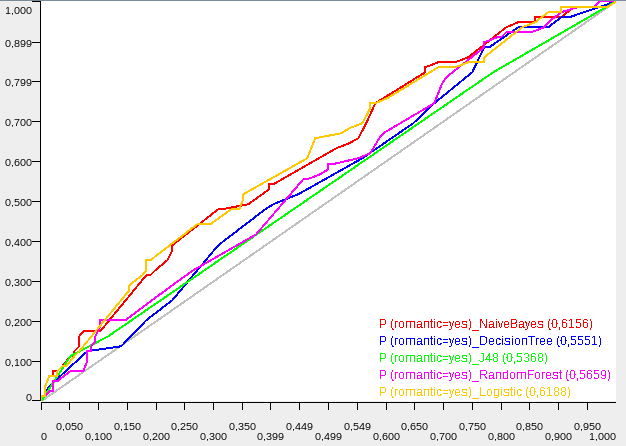
\includegraphics[width=1.02\linewidth]{RocCurve}}


\begin{center}
	\textit{Figure 1 - Roc Curve}
\end{center}

Di seguito vengono riportati i valori  AUC ottenuti dalla ROC curve. 

\begin{center}
	\begin{tabular}{|>{\centering\arraybackslash}m{3cm}|c|}
		\hline
		& AUC  \\
		\hline
		NaiveBayes & 0.616	\\
		\hline
		Decision Tree & 0.555   \\
		\hline
		J48 & 0.537  \\
		\hline
		Random Forest. & 0.566 \\
		\hline
		Logistic & 0.619 \\
		\hline
	\end{tabular}
\end{center}

Confrontando il grafico e i valori AUC ottenuti è possibile escludere Decision Tree, J48 e Random Forest che presentano valori dell'area sottesa alla curva più bassi. Mentre risulta difficile affermare con precisione quale classificatore, tra Logistic e Naive Bayes, sia il migliore. Qualora si dovesse preferire un modello si sceglierebbe il Naive Bayes in quanto presenta un valore di $F_1$-measure più alto.

 
\chapter{Conclusioni}

L’obiettivo che ci si era posti inizialmente, ovvero selezionare i modelli migliori in termini di performance e attendibilità per valutare quanto l’assunzione di alcolici potesse influire sulle possibilità di intraprendere una relazione romantica, non è stato perseguito. Di fatto la possibilità di valutare questo aspetto ha condotto alla generazione di un modello dove sono state messe in relazione le variabili “Dalc” e “Walc” (indipendenti) con la variabile “Romantic”. I risultati ottenuti hanno però dimostrato che i modelli non sono in grado di predire correttamente la variabile di classe utilizzando i due attributi riferiti all’alcool, ovvero di spiegare se una persona che assume alcool sia più o meno predisposta ad avere una relazione romantica. Per quanto, da un punto di vista scientifico, l’alcool sia ritenuto in grado di disinibire e di agire modificando i comportamenti naturalmente assunti dagli individui, questo non è correlabile con la variabile target “Romantic”.

A partire dall’esito ottenuto, si è ritenuto opportuno indagare ulteriormente cercando di capire quali variabili contenute nel dataset consentissero di ottenere performance migliori. Per questa ragione si è optato per una Feature Selection che ha confermato ulteriormente i risultati ottenuti in precedenza identificando nuove variabili. 

In generale si è ritenuto più affidabile utilizzare il metodo  dell’Iterated Holdout, rispetto all’Holdout classico, in quanto il limitato set di dati avrebbe portato un bias nei valori degli indici di performance.

I classificatori che risultano dall’Iterated Holdout applicato al modello con le variabili selezionate hanno un indice di performance $F_1$-measure più basso rispetto all’Iterated Holdout applicato al modello con tutti gli attributi a disposizione. I valori della Recall per la Feature Selection sono più bassi, ma ciò è legato al fatto che gli attributi usati siano solo 5, mentre nel caso del dataset completo si avevano a disposizione 32 variabili. Una bassa Recall indica che la classe rara non venga ben classificata (la nostra target). Inoltre i valori dell’Accuracy calcolata sui modelli con le sole variabili selezionate aumentano, ma in modo limitato, aspetto probabilmente causato dal fatto che la classe rara della variabile target sia leggermente sbilanciata.

Come anticipato tra i modelli realizzati tramite Feature Selection i più performanti risultano essere Naive Bayes e Logistic, nonostante ciò non si è in grado di stabilire quale sia il più appropriato. 

La scarsa numerosità del dataset ha influito sui risultati ottenuti e, in particolar modo, sulle misure di performance. Questa caratteristica ha condizionato molte scelte in fase di analisi dei dati in quanto diverse tecniche richiedevano ulteriori partizionamenti, impossibili da realizzare con sole 649 osservazioni. 

\end{multicols}
	
\end{document}